% Options for packages loaded elsewhere
\PassOptionsToPackage{unicode}{hyperref}
\PassOptionsToPackage{hyphens}{url}
\PassOptionsToPackage{dvipsnames,svgnames,x11names}{xcolor}
%
\documentclass[
  letterpaper,
  DIV=11,
  numbers=noendperiod]{scrartcl}

\usepackage{amsmath,amssymb}
\usepackage{lmodern}
\usepackage{iftex}
\ifPDFTeX
  \usepackage[T1]{fontenc}
  \usepackage[utf8]{inputenc}
  \usepackage{textcomp} % provide euro and other symbols
\else % if luatex or xetex
  \usepackage{unicode-math}
  \defaultfontfeatures{Scale=MatchLowercase}
  \defaultfontfeatures[\rmfamily]{Ligatures=TeX,Scale=1}
\fi
% Use upquote if available, for straight quotes in verbatim environments
\IfFileExists{upquote.sty}{\usepackage{upquote}}{}
\IfFileExists{microtype.sty}{% use microtype if available
  \usepackage[]{microtype}
  \UseMicrotypeSet[protrusion]{basicmath} % disable protrusion for tt fonts
}{}
\makeatletter
\@ifundefined{KOMAClassName}{% if non-KOMA class
  \IfFileExists{parskip.sty}{%
    \usepackage{parskip}
  }{% else
    \setlength{\parindent}{0pt}
    \setlength{\parskip}{6pt plus 2pt minus 1pt}}
}{% if KOMA class
  \KOMAoptions{parskip=half}}
\makeatother
\usepackage{xcolor}
\setlength{\emergencystretch}{3em} % prevent overfull lines
\setcounter{secnumdepth}{-\maxdimen} % remove section numbering
% Make \paragraph and \subparagraph free-standing
\ifx\paragraph\undefined\else
  \let\oldparagraph\paragraph
  \renewcommand{\paragraph}[1]{\oldparagraph{#1}\mbox{}}
\fi
\ifx\subparagraph\undefined\else
  \let\oldsubparagraph\subparagraph
  \renewcommand{\subparagraph}[1]{\oldsubparagraph{#1}\mbox{}}
\fi


\providecommand{\tightlist}{%
  \setlength{\itemsep}{0pt}\setlength{\parskip}{0pt}}\usepackage{longtable,booktabs,array}
\usepackage{calc} % for calculating minipage widths
% Correct order of tables after \paragraph or \subparagraph
\usepackage{etoolbox}
\makeatletter
\patchcmd\longtable{\par}{\if@noskipsec\mbox{}\fi\par}{}{}
\makeatother
% Allow footnotes in longtable head/foot
\IfFileExists{footnotehyper.sty}{\usepackage{footnotehyper}}{\usepackage{footnote}}
\makesavenoteenv{longtable}
\usepackage{graphicx}
\makeatletter
\def\maxwidth{\ifdim\Gin@nat@width>\linewidth\linewidth\else\Gin@nat@width\fi}
\def\maxheight{\ifdim\Gin@nat@height>\textheight\textheight\else\Gin@nat@height\fi}
\makeatother
% Scale images if necessary, so that they will not overflow the page
% margins by default, and it is still possible to overwrite the defaults
% using explicit options in \includegraphics[width, height, ...]{}
\setkeys{Gin}{width=\maxwidth,height=\maxheight,keepaspectratio}
% Set default figure placement to htbp
\makeatletter
\def\fps@figure{htbp}
\makeatother

\KOMAoption{captions}{tableheading}
\makeatletter
\makeatother
\makeatletter
\makeatother
\makeatletter
\@ifpackageloaded{caption}{}{\usepackage{caption}}
\AtBeginDocument{%
\ifdefined\contentsname
  \renewcommand*\contentsname{Table of contents}
\else
  \newcommand\contentsname{Table of contents}
\fi
\ifdefined\listfigurename
  \renewcommand*\listfigurename{List of Figures}
\else
  \newcommand\listfigurename{List of Figures}
\fi
\ifdefined\listtablename
  \renewcommand*\listtablename{List of Tables}
\else
  \newcommand\listtablename{List of Tables}
\fi
\ifdefined\figurename
  \renewcommand*\figurename{Figure}
\else
  \newcommand\figurename{Figure}
\fi
\ifdefined\tablename
  \renewcommand*\tablename{Table}
\else
  \newcommand\tablename{Table}
\fi
}
\@ifpackageloaded{float}{}{\usepackage{float}}
\floatstyle{ruled}
\@ifundefined{c@chapter}{\newfloat{codelisting}{h}{lop}}{\newfloat{codelisting}{h}{lop}[chapter]}
\floatname{codelisting}{Listing}
\newcommand*\listoflistings{\listof{codelisting}{List of Listings}}
\makeatother
\makeatletter
\@ifpackageloaded{caption}{}{\usepackage{caption}}
\@ifpackageloaded{subcaption}{}{\usepackage{subcaption}}
\makeatother
\makeatletter
\@ifpackageloaded{tcolorbox}{}{\usepackage[many]{tcolorbox}}
\makeatother
\makeatletter
\@ifundefined{shadecolor}{\definecolor{shadecolor}{rgb}{.97, .97, .97}}
\makeatother
\makeatletter
\makeatother
\ifLuaTeX
  \usepackage{selnolig}  % disable illegal ligatures
\fi
\IfFileExists{bookmark.sty}{\usepackage{bookmark}}{\usepackage{hyperref}}
\IfFileExists{xurl.sty}{\usepackage{xurl}}{} % add URL line breaks if available
\urlstyle{same} % disable monospaced font for URLs
\hypersetup{
  pdftitle={RD},
  pdfauthor={Hanno},
  colorlinks=true,
  linkcolor={blue},
  filecolor={Maroon},
  citecolor={Blue},
  urlcolor={Blue},
  pdfcreator={LaTeX via pandoc}}

\title{RD}
\author{Hanno}
\date{}

\begin{document}
\maketitle
\ifdefined\Shaded\renewenvironment{Shaded}{\begin{tcolorbox}[frame hidden, breakable, borderline west={3pt}{0pt}{shadecolor}, interior hidden, boxrule=0pt, sharp corners, enhanced]}{\end{tcolorbox}}\fi

\hypertarget{main-rd-results}{%
\section{Main RD results}\label{main-rd-results}}

\hypertarget{optimal-bws-for-each-outcome-subset}{%
\subsection{Optimal BWs for each outcome /
subset}\label{optimal-bws-for-each-outcome-subset}}

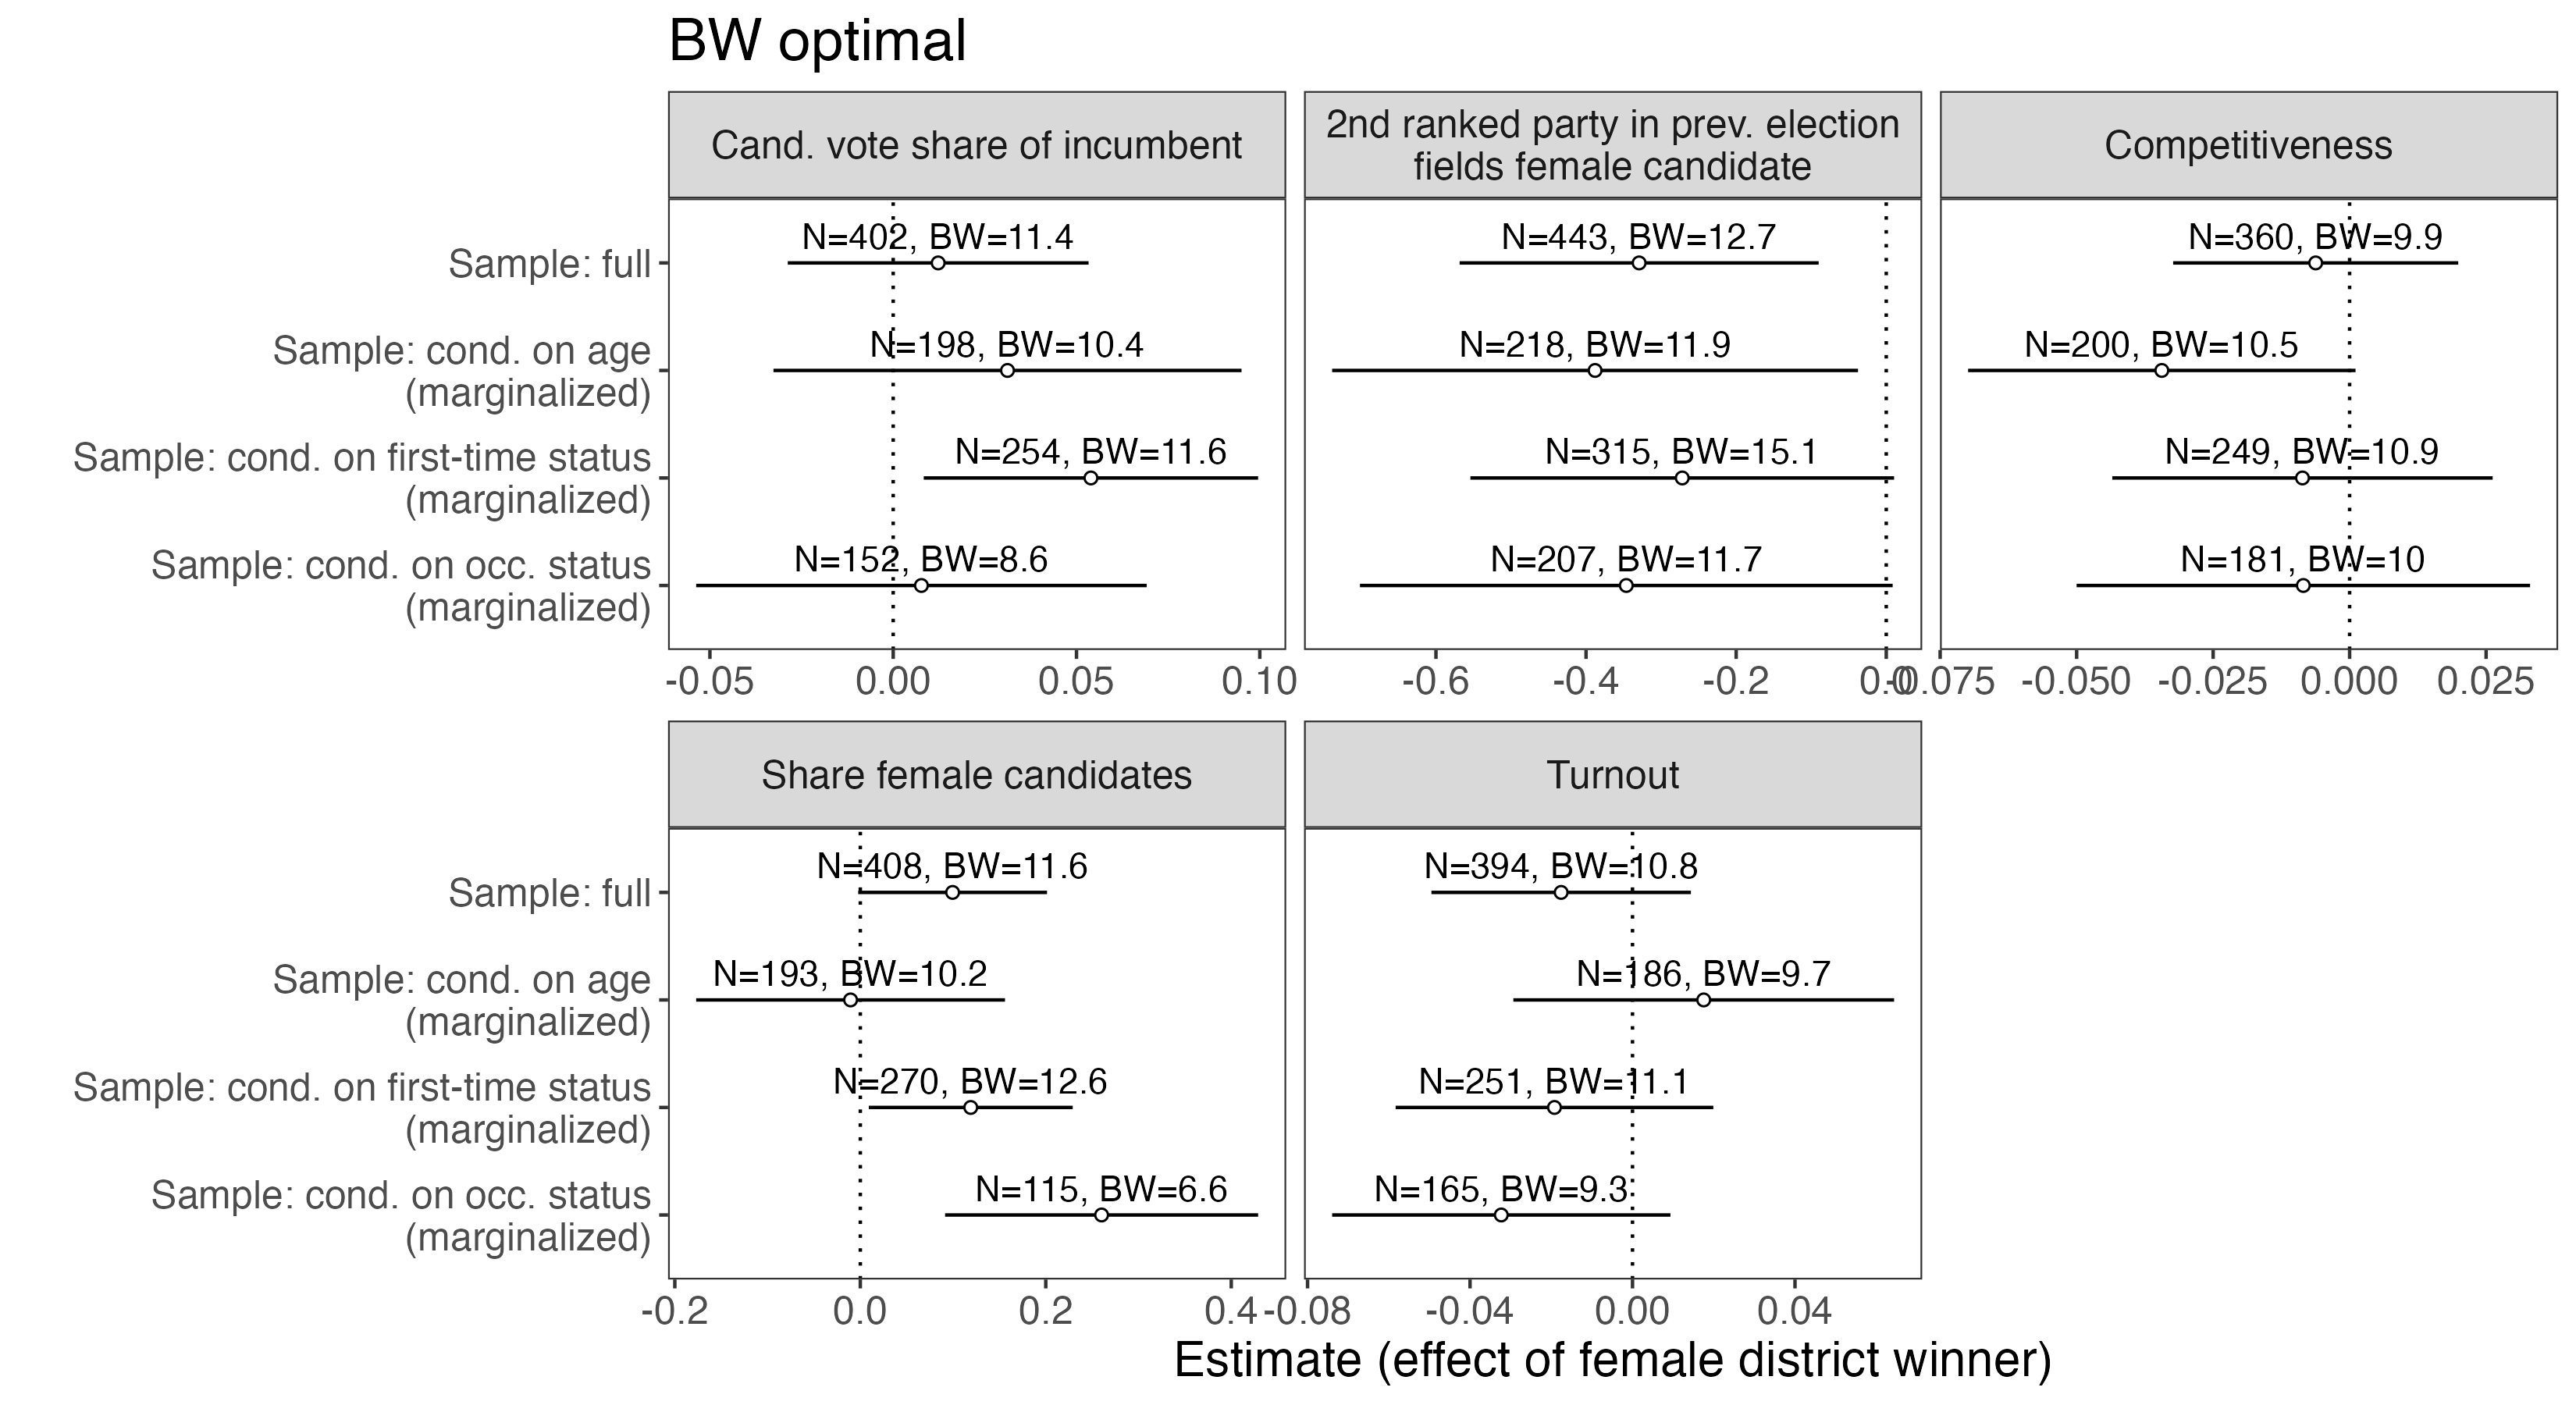
\includegraphics{images/Res_GER_Districts_marg.png}

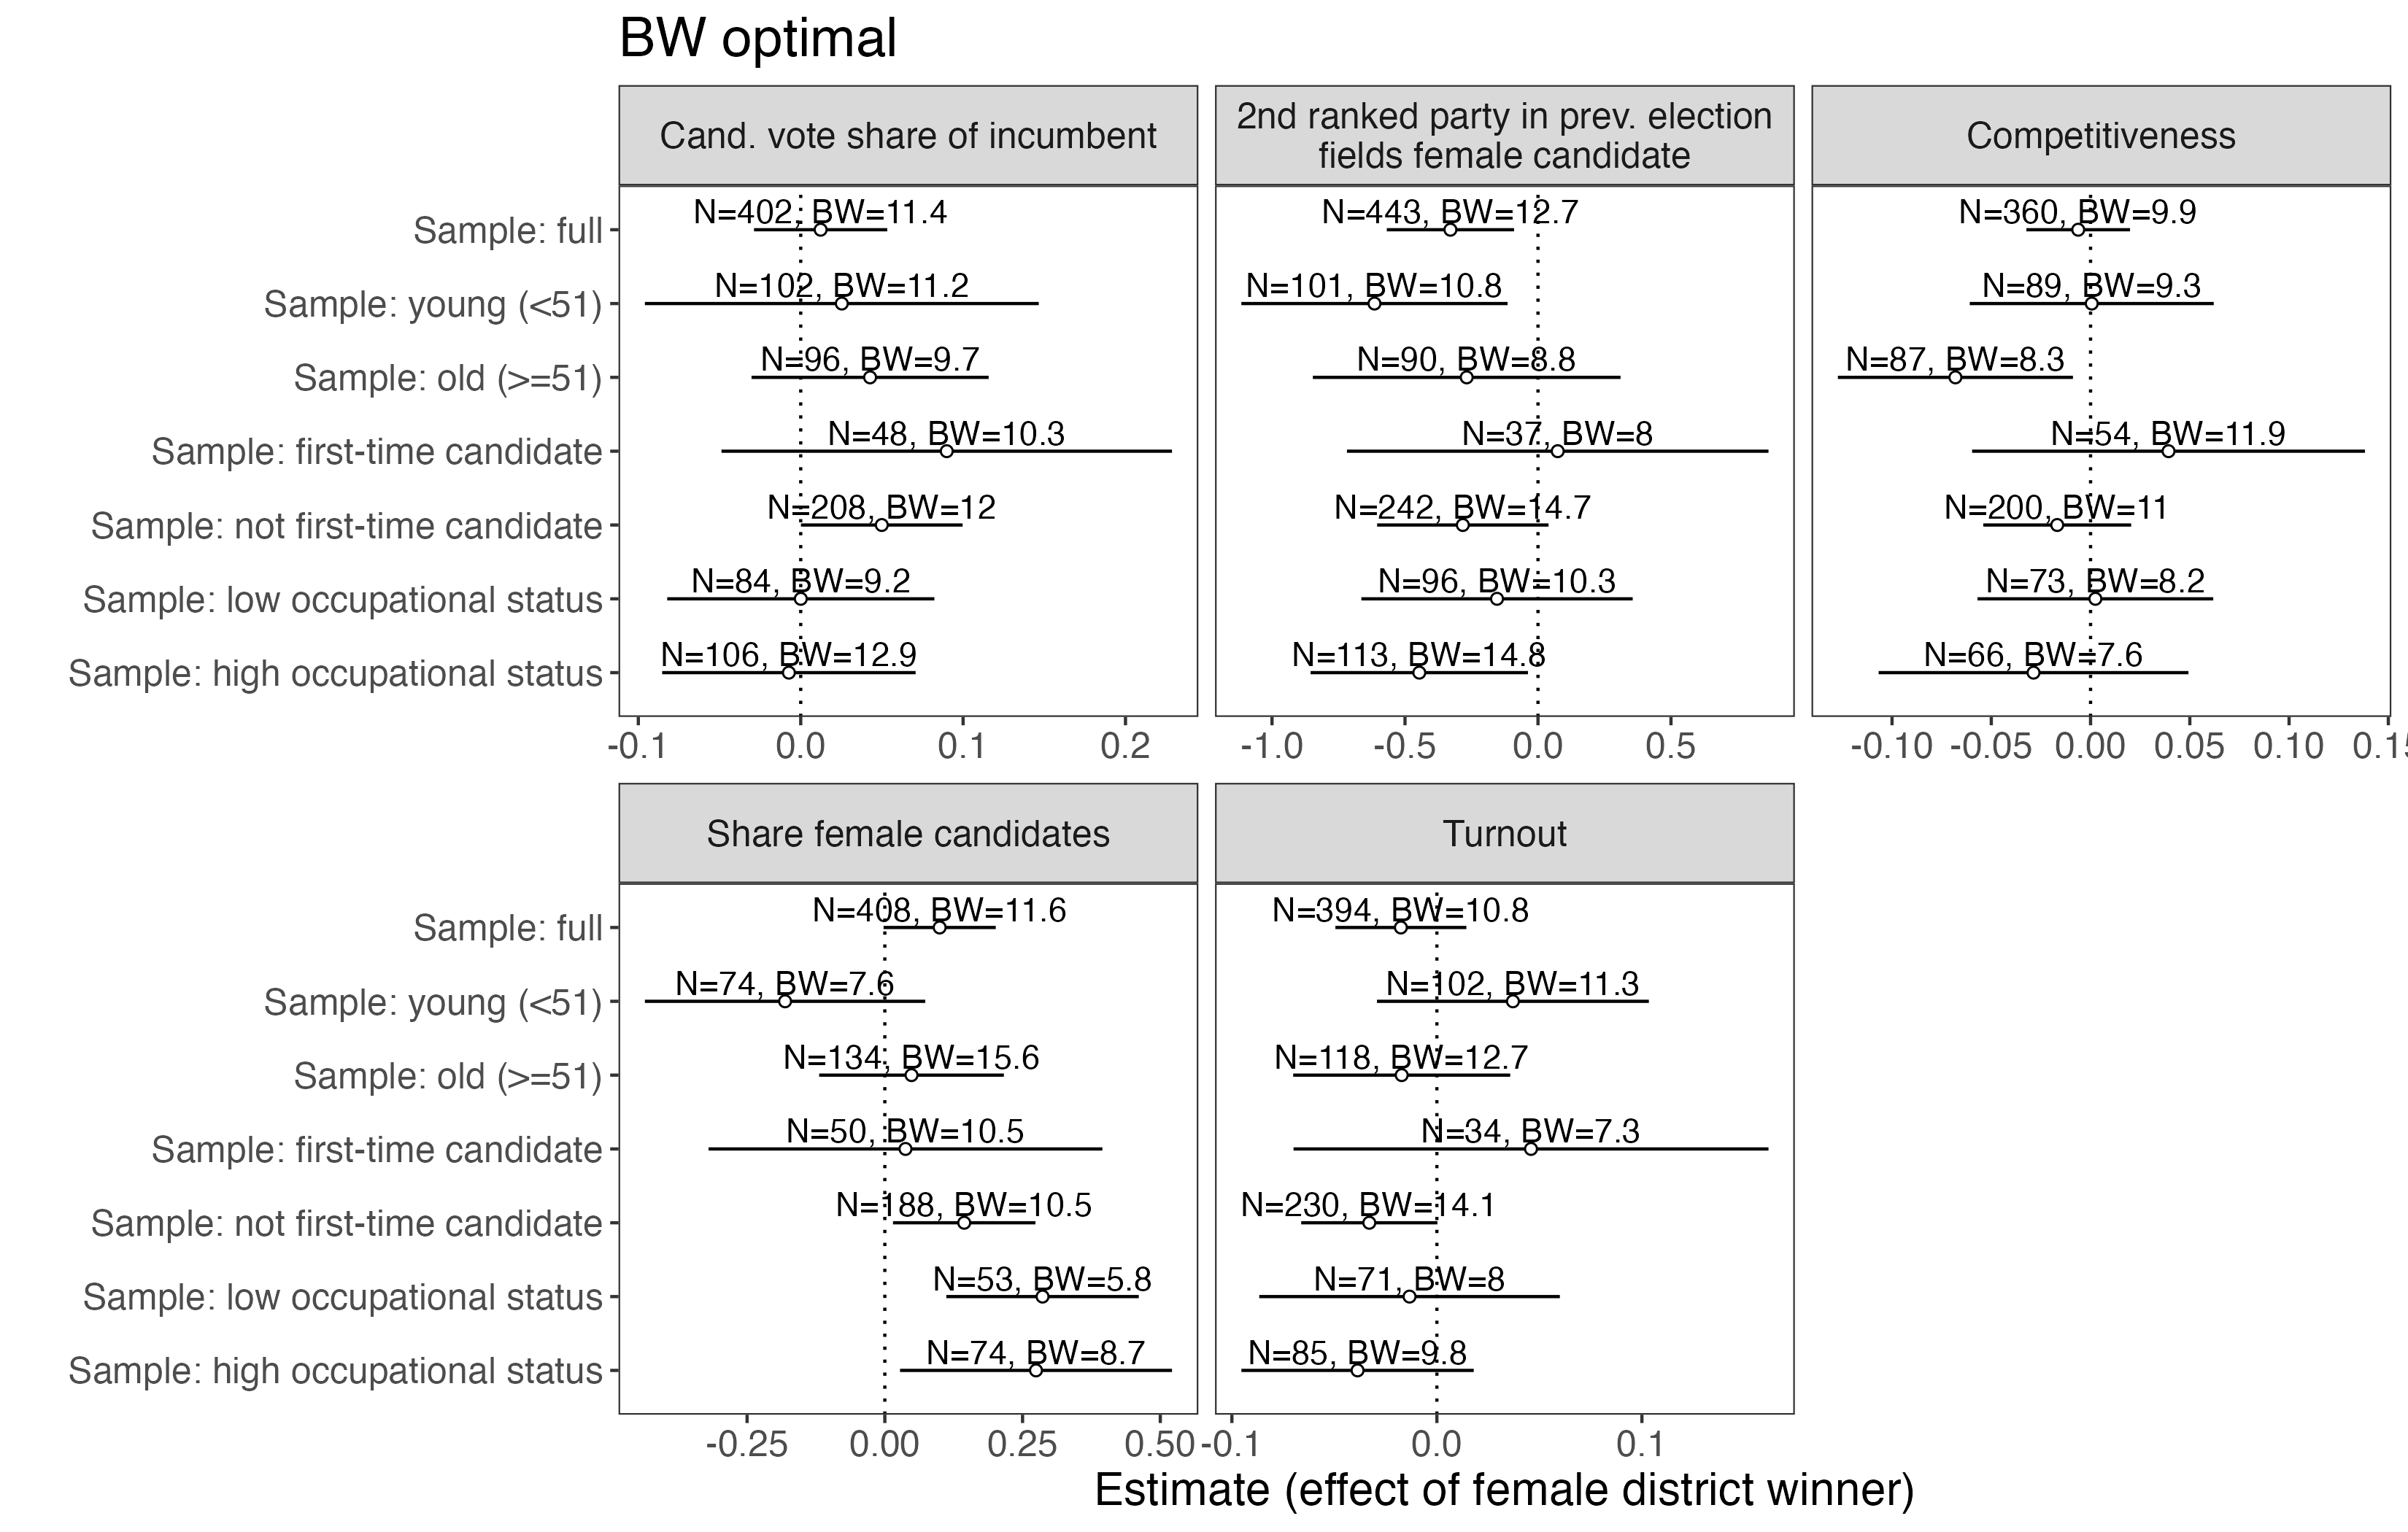
\includegraphics{images/Res_GER_Districts_cond.png}

\hypertarget{balance}{%
\section{Balance}\label{balance}}

\hypertarget{across-districts}{%
\subsection{Across districts}\label{across-districts}}

This compares female to male district winners, conditional on the
difference in vote shares. This is for the subset of opposite-gender
races.

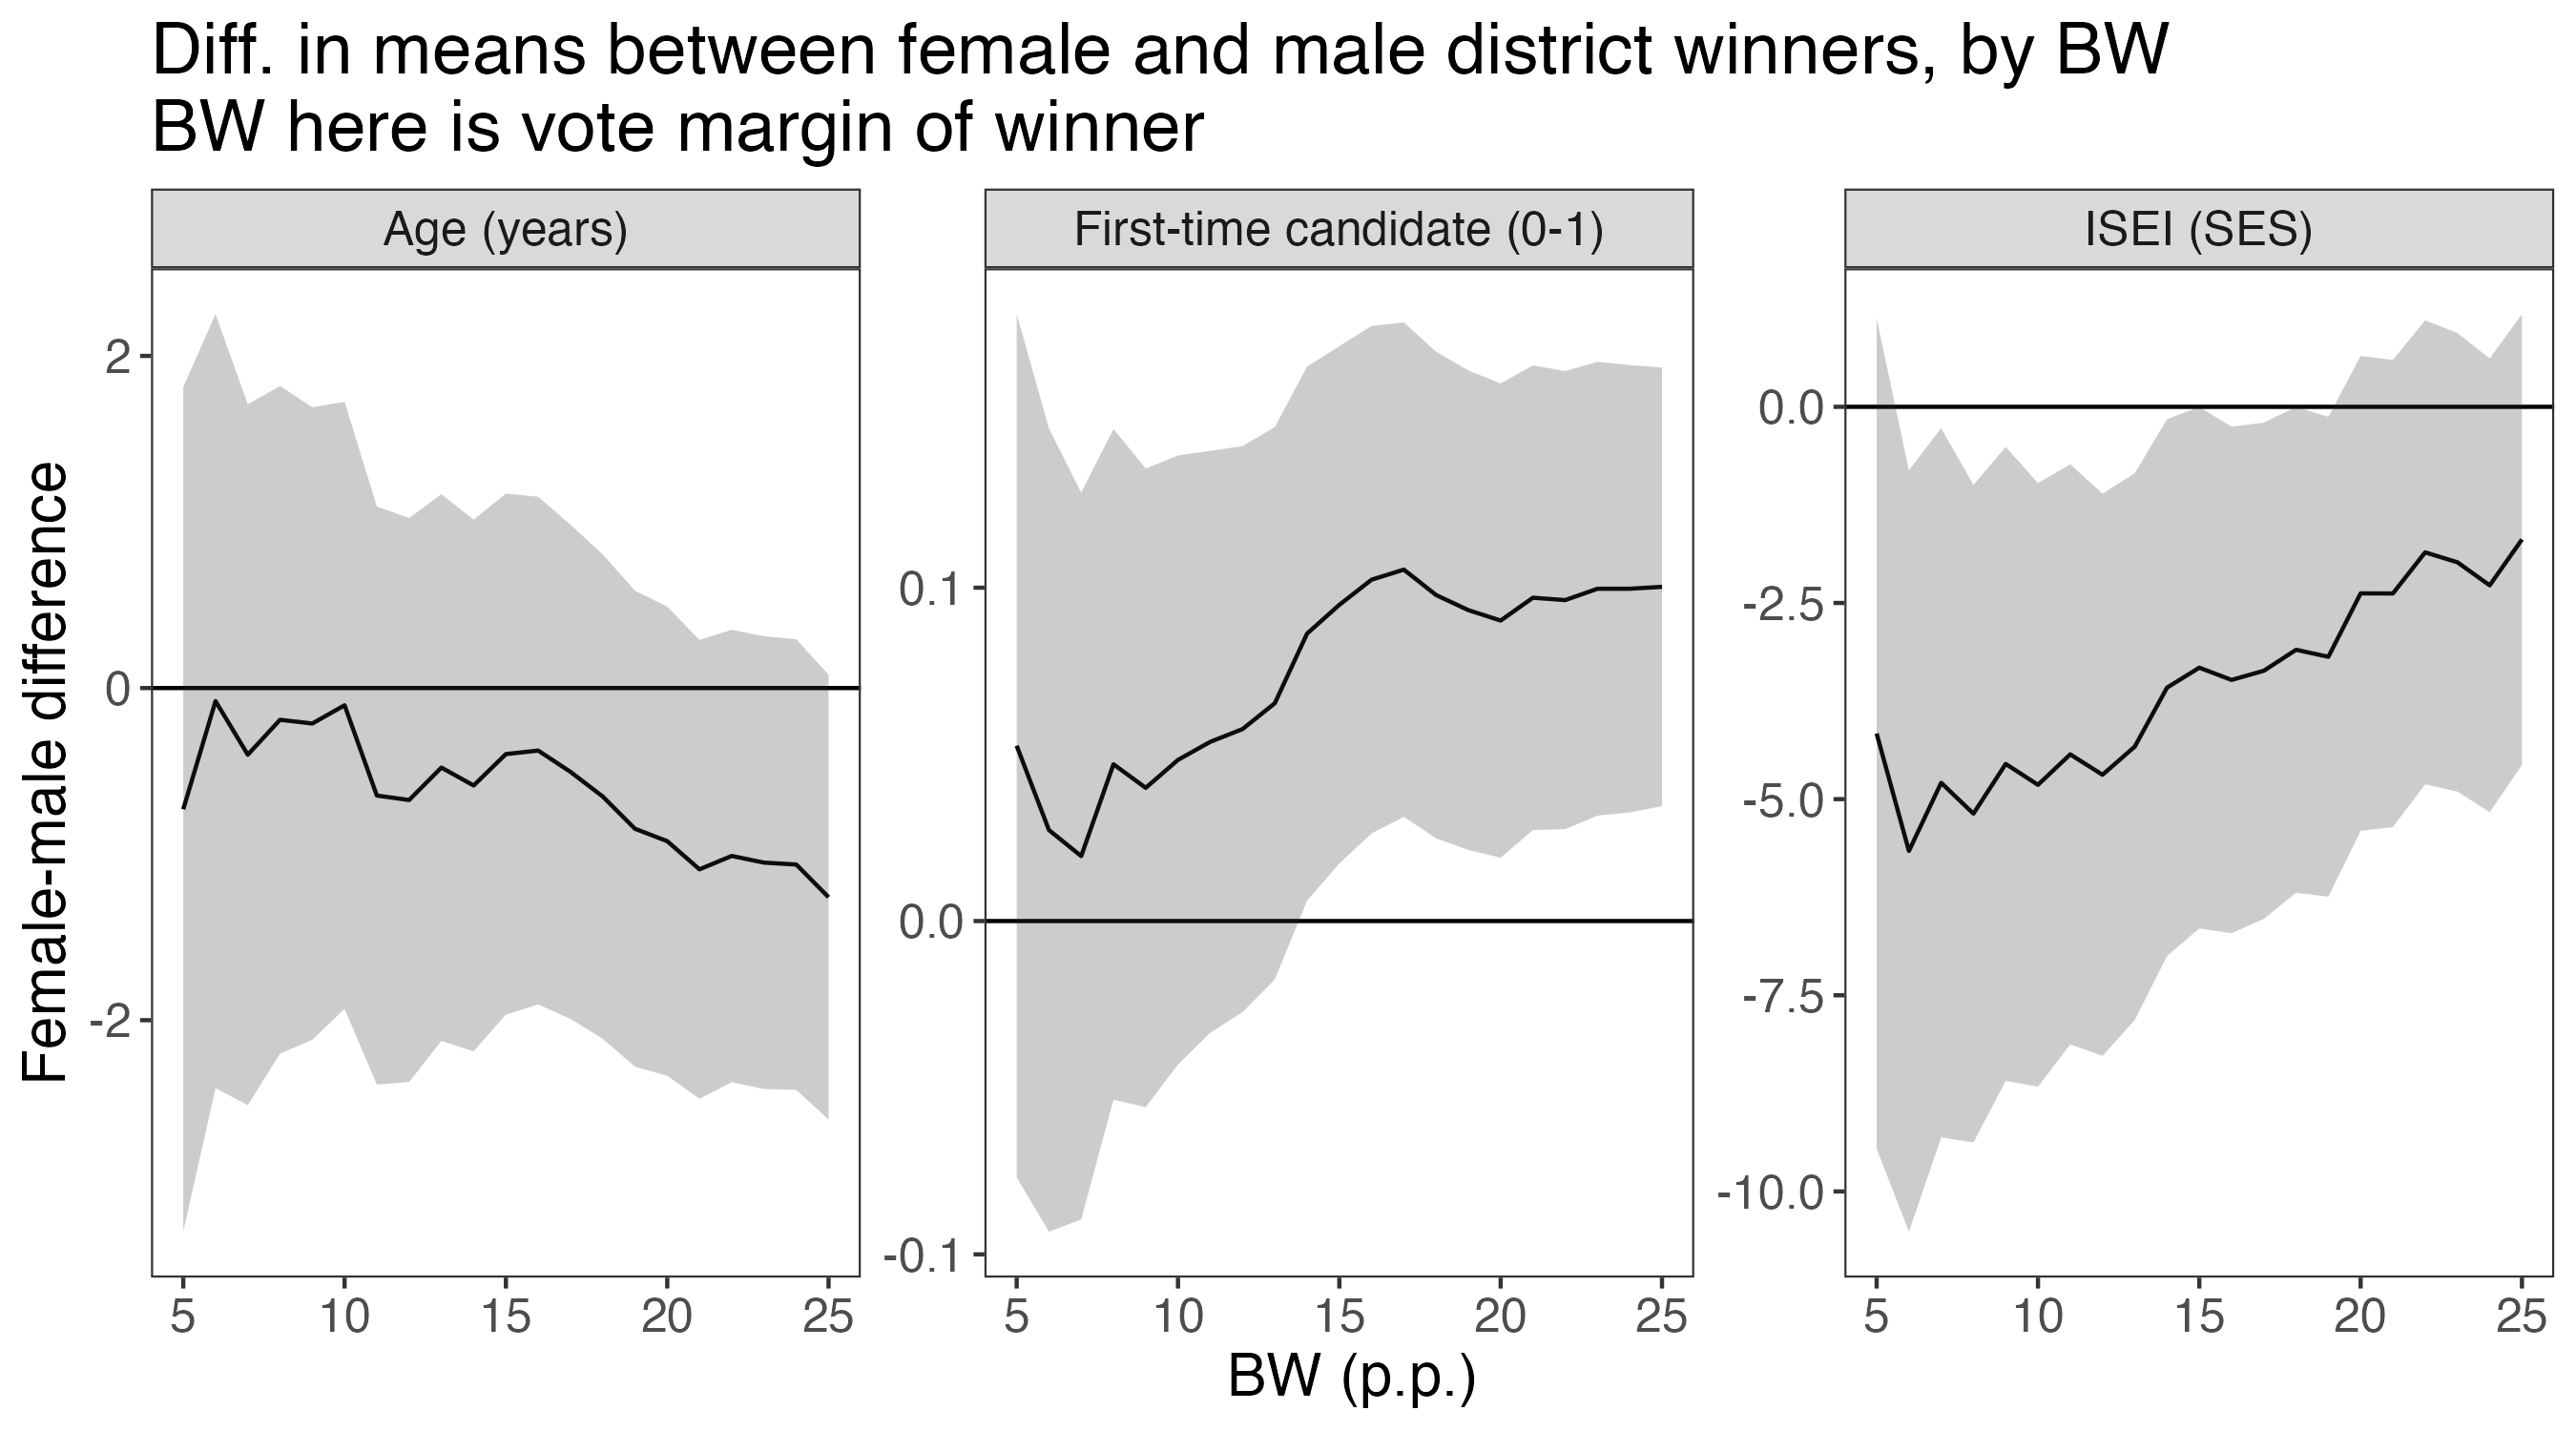
\includegraphics{images/Balance_AcrossDist.png}

\hypertarget{within-districts}{%
\subsection{Within districts}\label{within-districts}}

This compares female to male \emph{candidates}, i.e.~the first and
second ranked candidates in each district. The sample is limited to
opposite-gender races. Results are conditional on the difference in vote
shares between the first and second ranked candidates.

Subsets are defined by gender of election winner (first column is
results independent of election winner).

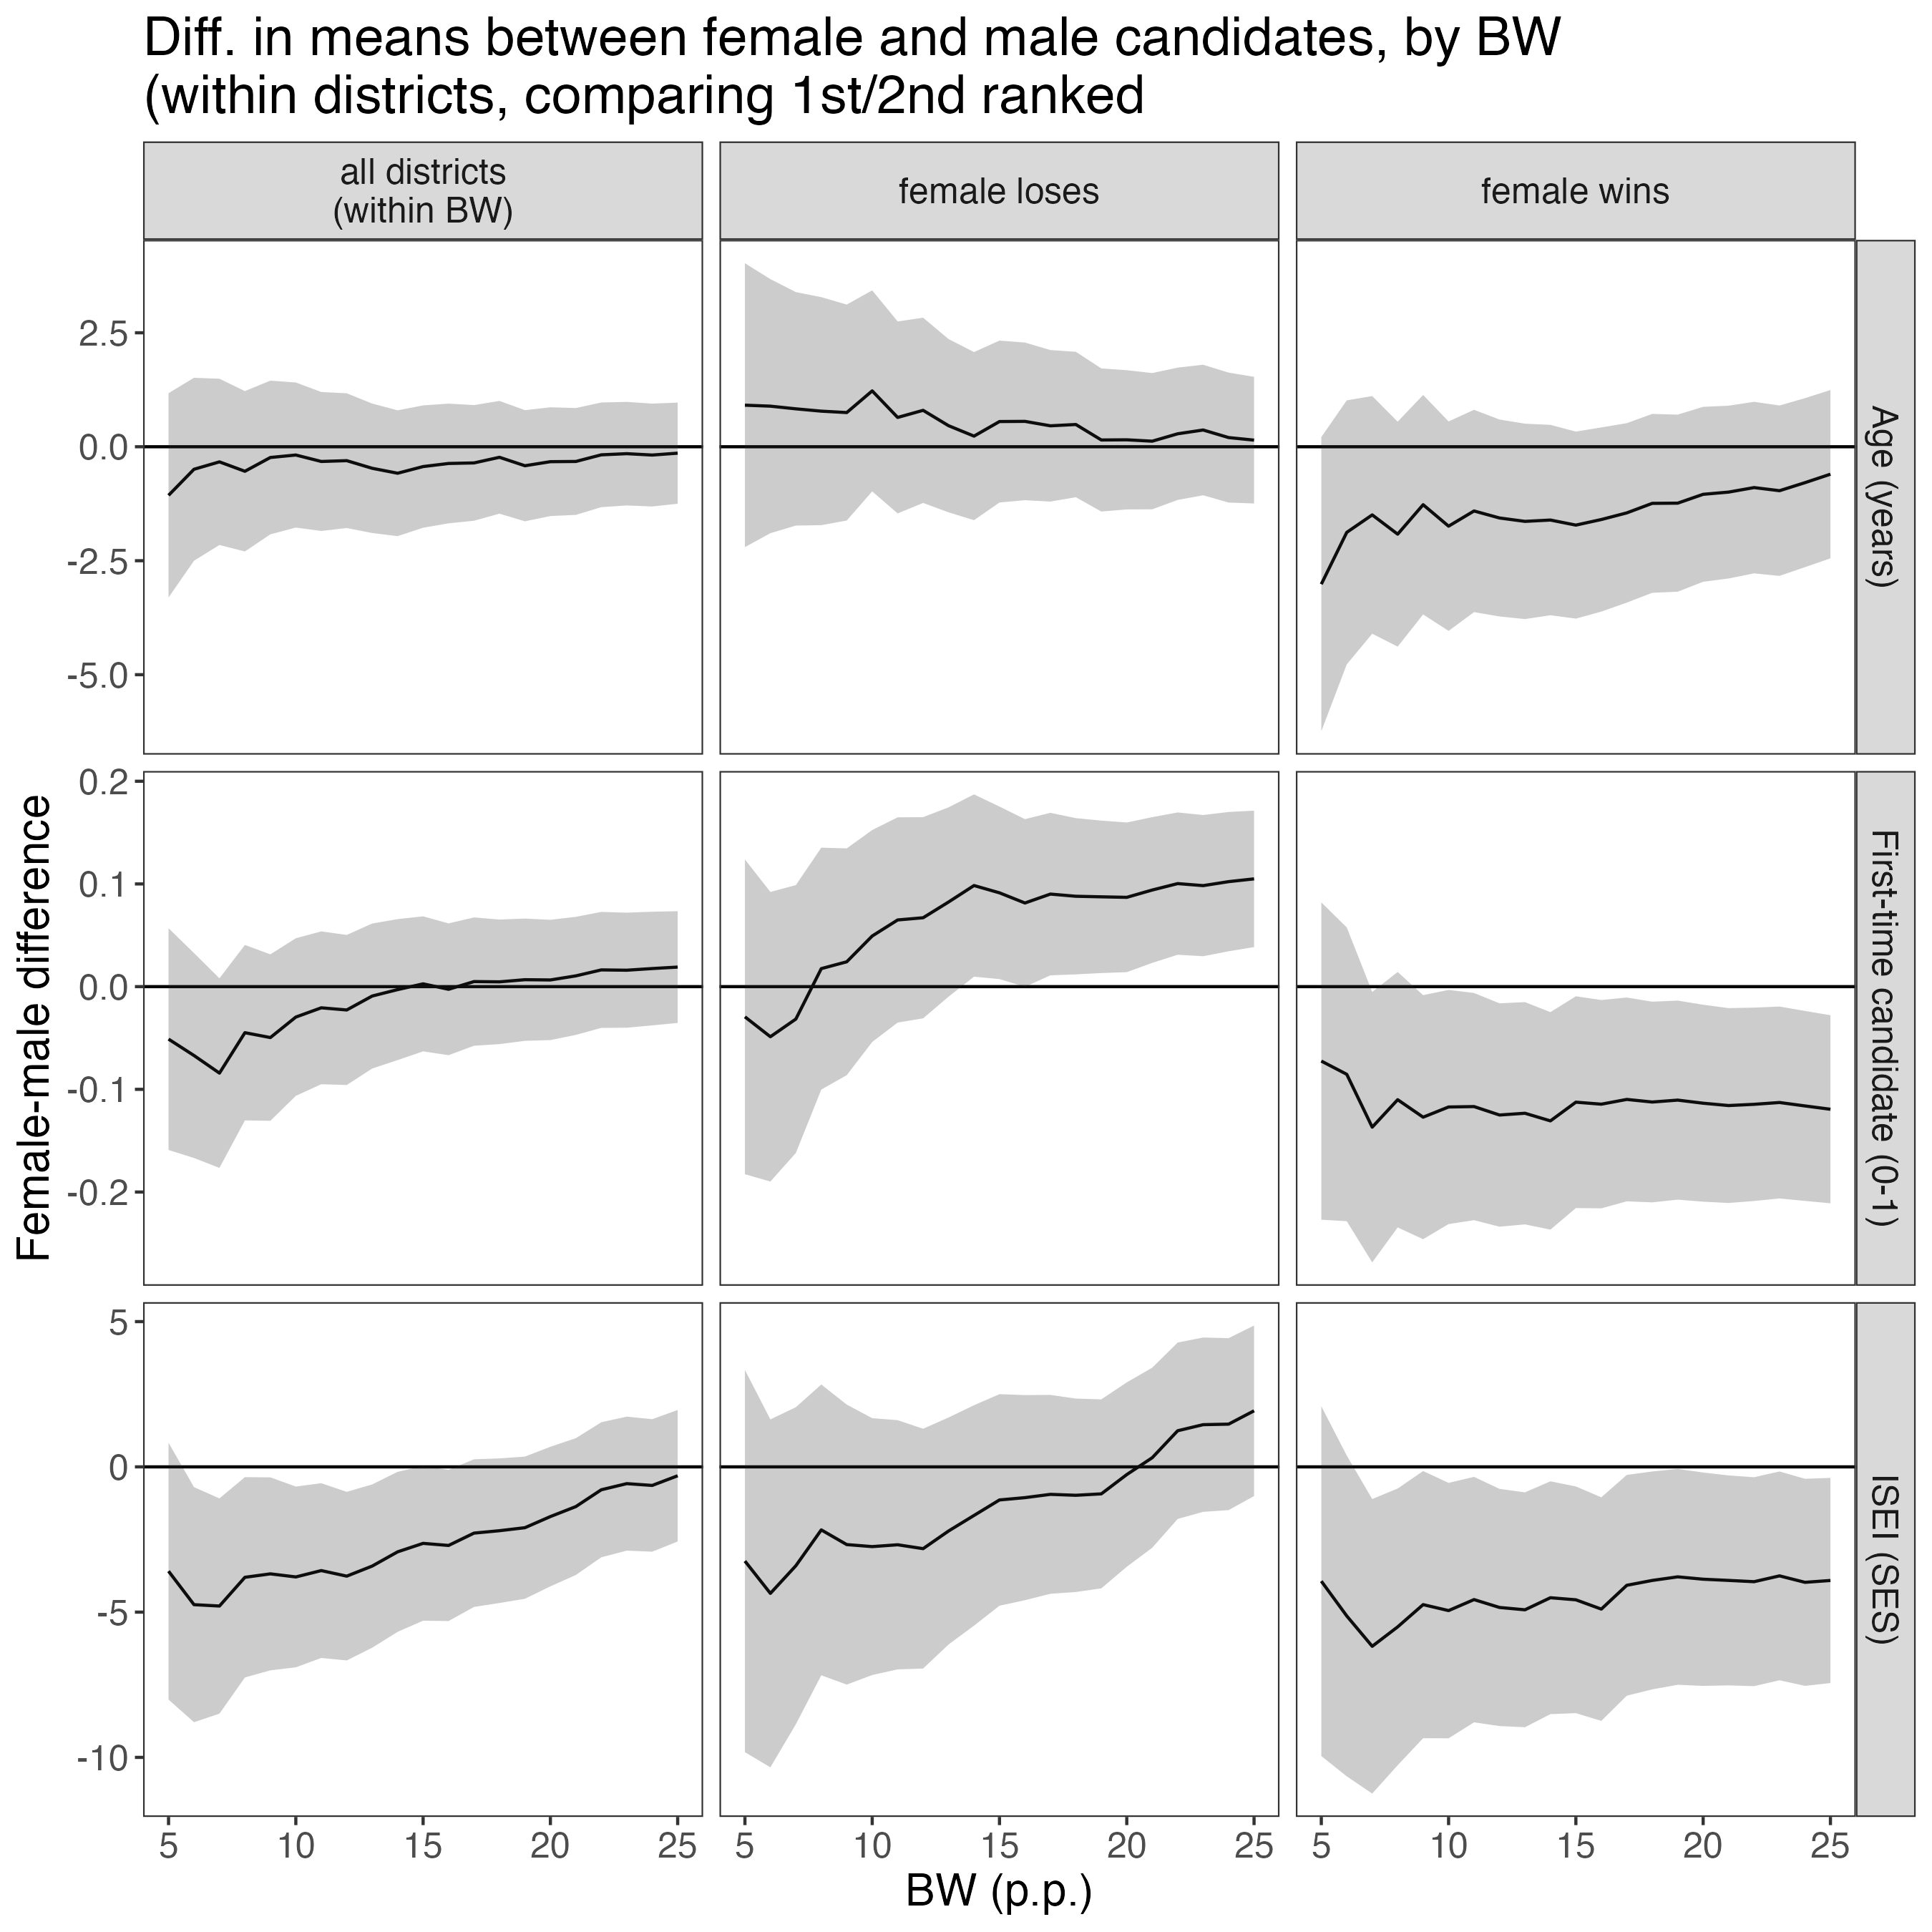
\includegraphics{images/Balance_WithinDist.png}

\hypertarget{number-of-observations-if-we-extend-data-backwards}{%
\section{Number of observations if we extend data
backwards}\label{number-of-observations-if-we-extend-data-backwards}}

This is cumulative number of observations conditional on number of
elections (i.e.~increases the further back in time we go) -- this is
already for the sample of races with opposite-gender candidates and
within 13p.p. bandwidth.

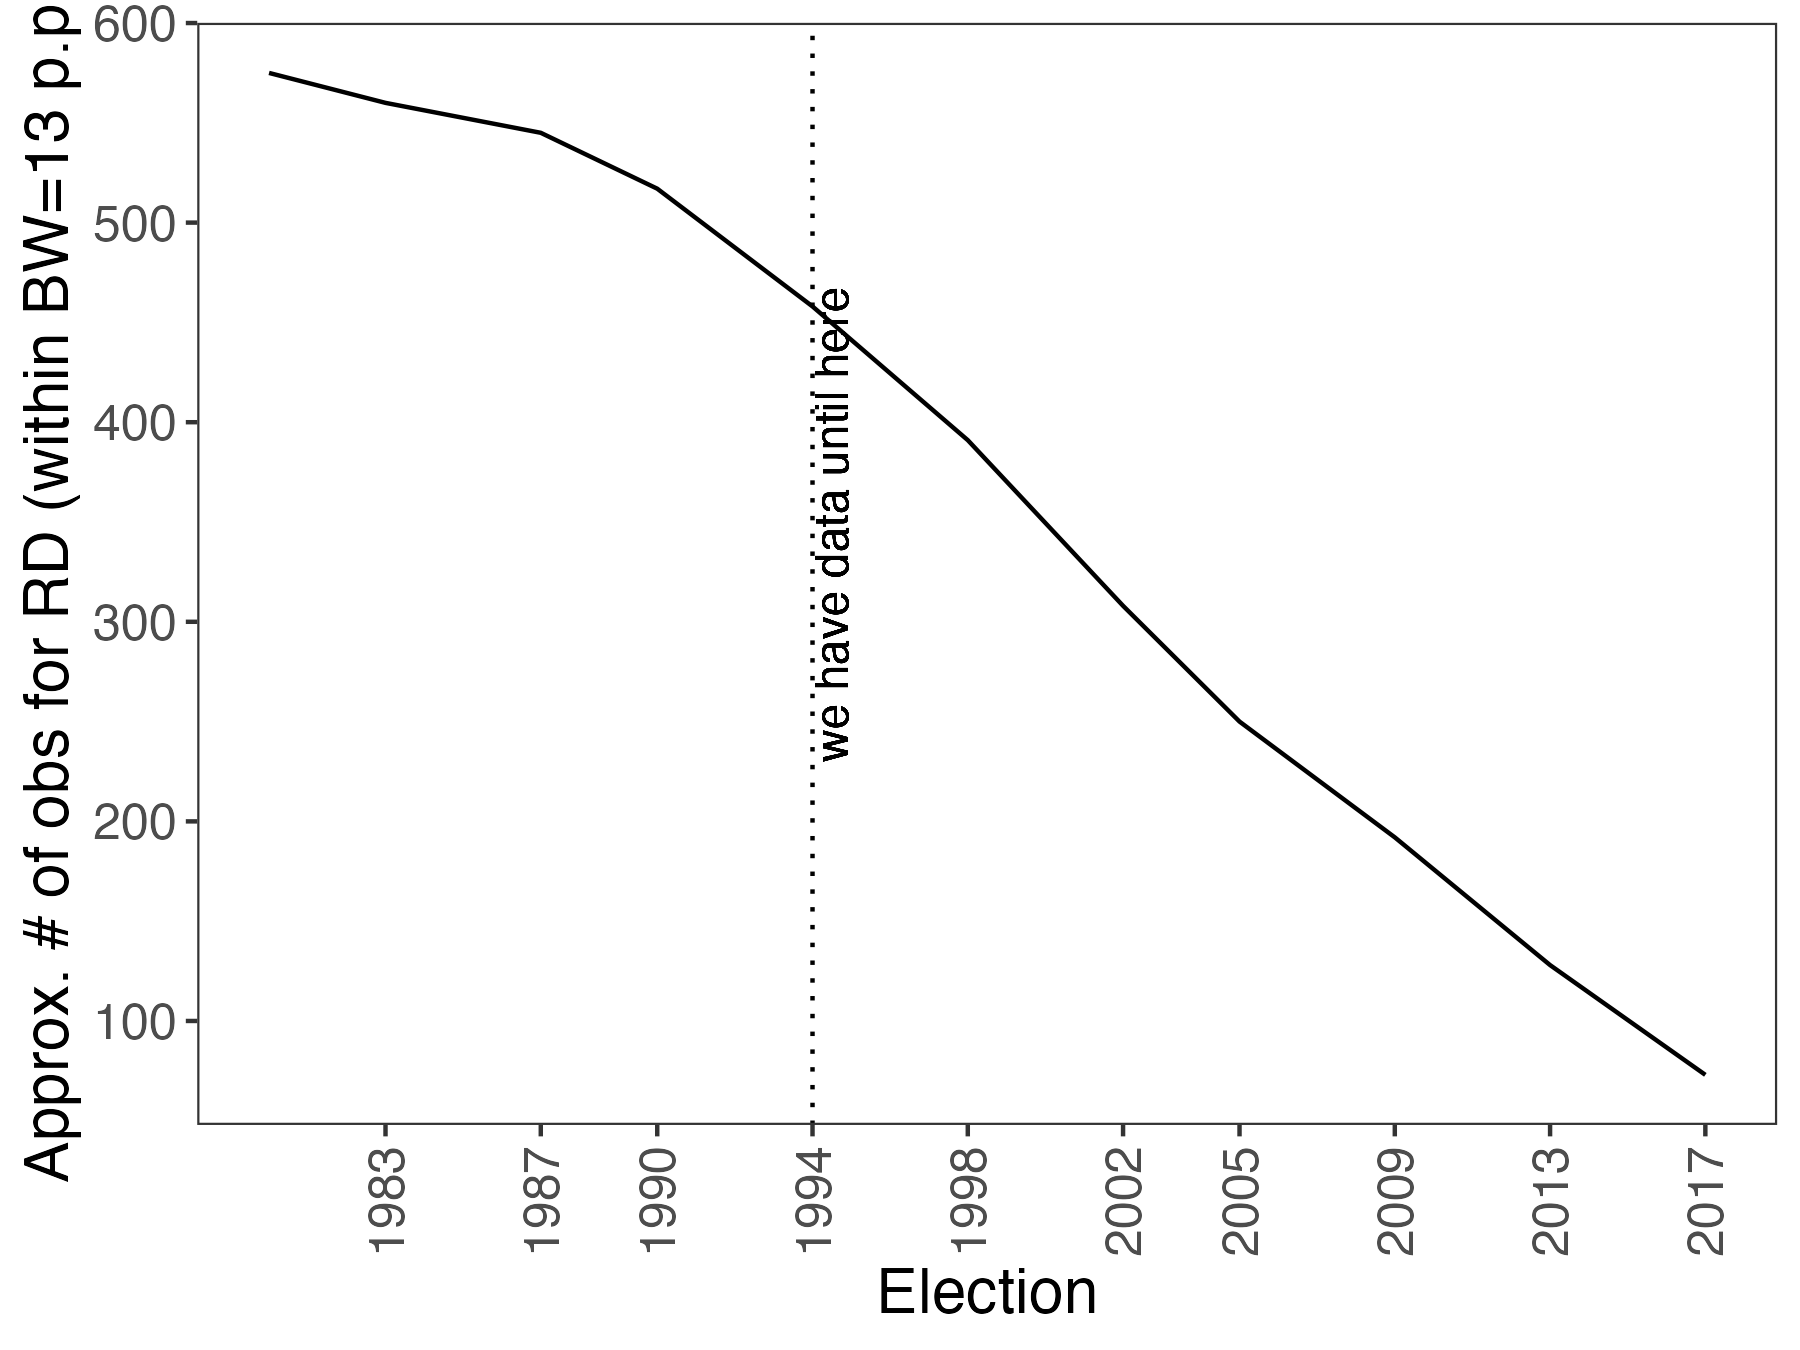
\includegraphics{images/Obs.png}

\hypertarget{more-info}{%
\section{More info}\label{more-info}}

\begin{itemize}
\tightlist
\item
  \textbf{Setting:} SMD races in German federal elections

  \begin{itemize}
  \tightlist
  \item
    5 (6 after 2013) main parties always field candidates in all
    districts in all elections
  \item
    Voters vote for one candidate, candidate who wins a plurality of
    vote goes to parliament
  \item
    No term limits
  \item
    Mixed system: 50\% of candidates are elected in districts, 50\% are
    elected through party lists (candidates can be nominated in
    districts and be on the list)
  \end{itemize}
\item
  \textbf{Sample:} SMDs in federal elections, 2002-2021 (6 elections)

  \begin{itemize}
  \tightlist
  \item
    Subset to races where top-2 candidates are of opposite gender
  \end{itemize}
\item
  \textbf{Treatment:} female candidate won in prev. election in the same
  districts
\item
  \textbf{Running variable:} defined as difference between female and
  male candidate in prev. election
\item
  \textbf{Specification:} No covariates, SEs clustered by electoral
  districts

  \begin{itemize}
  \tightlist
  \item
    Not sure if clustering makes sense here, could also not do this
  \item
    Could add election FEs / State FEs as covars?
  \end{itemize}
\item
  \textbf{Outcomes:}

  \begin{itemize}
  \tightlist
  \item
    Turnout (0-1)
  \item
    Share female candidates in the district (0-1) (of the 5/6 main
    parties)
  \item
    Competitiveness: vote share difference between first and
    second-ranked candidate (0-1)

    \begin{itemize}
    \tightlist
    \item
      Similar to running variable
    \end{itemize}
  \item
    `Incumbent candidate' vote share (0-1)

    \begin{itemize}
    \tightlist
    \item
      Assume candidate of party \(p\) wins in district \(j\) in election
      \(t\). This is the vote share of the candidate of party \(p\) in
      district \(j\) in election \(t+1\), regardless of whether party
      \(p\) fields the same candidate again or not.
    \end{itemize}
  \item
    2nd ranked party in prev election fields female candidate (0/1)

    \begin{itemize}
    \tightlist
    \item
      Assume party \(p\) is ranked second in district \(j\) in election
      \(t\). This measures whether party \(p\) fields a female candidate
      in election \(t+1\)
    \end{itemize}
  \end{itemize}
\end{itemize}

\textbf{Subsetting:} this is always based on top two candidates in the
previous election, i.e.~the condition (eg ``young candidate'') needs to
hold for both candidates - This means that there is a ``missing'' subset
of districts that are not covered by the subsets, ie districts for which
the condition only holds for one of the two candidates

\textbf{Bandwidths:} I show this forseparate optimal BWs by sample

\textbf{Extending data backwards:} We could extend this backwards,
however there are no shapefiles for districts prior to 1998 (as far as I
can tell) -- we need shapefiles to keep track of redistricting over
time.

\textbf{Exclusion due to redistricting:} I use shapefiles to track
redistricting, and I exclude districts that are less than 90\% the same
as in the previous election (happy to explain what that means)

\textbf{Potential other outcomes:} - Total voteshare of left-leaning
parties - Binary measures of fielding female candidate by party



\end{document}
